%
% IEEE Transactions on Microwave Theory and Techniques example
% Tibault Reveyrand - http://www.microwave.fr
%
% http://www.microwave.fr/LaTeX.html
% ---------------------------------------



% ================================================
% Please HIGHLIGHT the new inputs such like this :
% Text :
%  \hl{comment}
% Aligned Eq. 
% \begin{shaded}
% \end{shaded}
% ================================================



\documentclass[journal]{IEEEtran}

%\usepackage[retainorgcmds]{IEEEtrantools}
%\usepackage{bibentry}  
\usepackage{xcolor,soul,framed} %,caption

\colorlet{shadecolor}{yellow}
% \usepackage{color,soul}
\usepackage[pdftex]{graphicx}
\graphicspath{{../pdf/}{../jpeg/}}
\DeclareGraphicsExtensions{.pdf,.jpeg,.png}

\usepackage[cmex10]{amsmath}
%Mathabx do not work on ScribTex => Removed
%\usepackage{mathabx}
\usepackage{array}
\usepackage{mdwmath}
\usepackage{mdwtab}
\usepackage{eqparbox}
\usepackage{url}
\usepackage{lipsum}
\usepackage{booktabs}
\usepackage{rotating}
\usepackage{graphicx}
\usepackage{multicol}
\usepackage{multirow}
\usepackage{listings} % code blocks

\lstset{
  basicstyle={\small\ttfamily},
  breaklines=true,
  breakatwhitespace=true,
  tabsize=2
}


%\bstctlcite{IEEE:BSTcontrol}


%=== TITLE & AUTHORS ====================================================================
\begin{document}
\title{Fast Network Threat Detection based on the TRAbID dataset: An Analysis of Various Machine Learning Models }
\author{
Shrey Agarwal,
Ashwini Hiremath,
Ibrahim Khalid,
Harsh Shinde,
Justin Wang%
\thanks{Dr. Shih Yu Chang}
}
% The paper headers
\markboth{Fast Network Threat Detection}{Fast Network Threat Detection}


\maketitle



\begin{abstract}
one sentence on problem, couple sentences on process, one or two sentences with the results
\end{abstract}

\begin{IEEEkeywords}
Network anomaly detection, Machine Learning
\end{IEEEkeywords}

\IEEEpeerreviewmaketitle



% === I. INTRODUCTION =============================================================
% =================================================================================
\section{Introduction}

\IEEEPARstart{I}{n} our ever increasing digital world, it is vital that we also have improved security over our networks. Based on the Cloudflare DDoS 2023 Q4 report \cite{cloudflare} and Verizon’s data breach report 2023 \cite{verizion}, there has been an increase in the number of cyber attacks, including network based attacks. By using live network data and classifying it as harmful or not, we can create a system that will improve the peace of mind of a user and allow them to use modern technology with confidence.

The primary objective of this project is to train various machine learning models for the classification of whether an activity on the network is a threat or not. The secondary objective of this project is to evaluate the machine learning models based on their performance, and computation time and cost in order to find the best model. This can be used to create a firewall application \cite{ucar2017analysis} that uses the built machine learning model.

\section{Literature review}
Bagui et al. explored the UNSW-NB15 dataset using a hybrid approach that used k-means clustering followed by decision trees or Naive Bayes. Using decision trees, they were able to achieve a 99\% accuracy rate. \cite{bagui2019using} Bhati et al. used the KDDCUP99 dataset to explore the effectiveness of ensemble models such as AdaBoost and Random Forest. \cite{bhati2022ensemble} 

Zhou and Yang  developed an ``immune algorithm'' for detecting network anamolies using SVM. They were able to find that using such an algorithm, they were able to get an accuracy of 94\% with a detection time of 27 seconds for the entire test suite. \cite{zhou2006using}

Tavallaee et al. developed multiple machine learning models trained on the KDDCUP99 dataset, including Random Forest, Naive Bayes, and SVM. They were able to get accuracies of 92.8\%, 81.7\%, and 65.1\%, respectively. \cite{tavallaee2009detailed}

Viegas et al. generated the TRAbID dataset with the goal of providing a better dataset for training machine learning models. They trained on this dataset using the Naive Bayes and Decision Tree algorithms. \cite{viegas2017toward}

Based on our short literature review among the listed papers and otherwise, there has not been a clear strive for creating a model with the goal of fast detection after training. We plan on furthering research in this regard by exploring the effectiveness of various machine learning techniques on the TRAbID dataset.

\section{Proposed methodology}
We are planning to use the TRAbID dataset \cite{viegas2017toward} as it provides a relevant dataset for the problem, this can be subject to change. The TRAbID dataset is sufficiently large, with 44 feature columns, including classification, made up of generated network traffic data. Our methodology will be to first explore this dataset using tools such as Pandas, MatPlotLib, and Sci-Kit Learn. This includes tasks such as identifying correlations, normalizing values, and selecting important features. Following this, we will work on training a few different types of models in order to determine which models perform the best at distinguishing network threats. Models we plan on training are: Support Vector Machines, Logistic Regression, Naive Bayes, Random Forest, and XGBoost. These selected models can be subject to change. We will compare the models based on accuracy, precision and recall, and speed of classification.

\subsection{Hypothesis}
The anticipated results include improved organizational knowledge and awareness of the cyber threat landscape, allowing for improved readiness and response tactics. Furthermore, by adding to the body of knowledge on cybersecurity, these assessments hope to enhance defense systems and policies. The expected outcome of this research is to find a model that is able to quickly and accurately classify network traffic data. Future work based use cases on this research project would be to create a live network monitoring firewall application that can quickly run network traffic through a trained model and notify the user in case of a network based attack.

\section{Data Process}
% Should we ref the website we got it from
The dataset was downloaded from the original source as `arff' files. These files were quite large consisting of nearly 28,000,000 rows. Moreover, there was a huge imbalance in the dataset with nearly 99.7\% of the entries being `normal' entries. In order to reduce the computational complexity of this project as well as fix the class imbalance, we used a shell script to reduce the dataset 

\section{Data Understanding and Exploration}
% For data undersstanding, we can prob have a quick paragraph describing the data

% Potentially stuff like the null values and so on
% correlation
% VIF
% PCA

% based on rubric, we also may need explanations about the relationships between the EDA results and our problem statement
% Rubric has a data preperation/preprocessing step; should we shoehorn it into this since our reasoning is also here, or should we make a new section?

\section{Designing benchmark}


\section{Modelling}
\subsection{Naive Bayes}
% Probably can include how naive bayes works, showing equations and what not
Naive Bayes is a supervised learning technique that is based on the Naive Bayes theorem. Unlike the other models in this report (SVM, Logistic Regression, and the tree based models), Naive Bayes is considered as a generative learning algorithm, focusing to model the distribution of inputs of a given class rather than learning which features are most important for discrimination. Some advantages of Naive Bayes include its simplicity and efficiency, the ability to handle high dimensional data, and its scalability. Some disadvantages include its assumption of conditional independence which causes to to be unrealistic, as well as its subjectability to the ``Zero Frequency'', which occurs when a feature does not exist in the training, causing the model to only predict zero.

For the modeling step, ComplementNB(), which is a version of MultinomialNB() that was designed to correct some its severe assumptions and works well with imbalanced data, as well as GaussianNB() was used. Additionally, hyperparameter tuning using GridSearchCV was utilized in order to improve results. ComplementNB() and GaussianNB() have different parameters, so they will be gone over in their sections.

\subsubsection{Complement Naive Bayes}
Complement Naive Bayes is a variation of Multinomial Naive Bayes that uses the complement of each class to calculate weights. As a result, this makes this model more suitable for imbalanced datasets, such as the TRAbID dataset. Complement Naive Bayes has the following parameters: alpha, force\_alpha, fit\_prior, class\_prior, and norm. Alpha is the smoothing parameter, force\_alpha will set alpha to 1e-10 if it is too low, fit\_prior is only used in edge cases with a single classes in the data, class\_prior is the prior probabilities of the classes but is not used in this implementation, and norm performs a second normalization of the weights. The parameter grid is as follows: 
% \{
%     "alpha": [0.001, 0.01, 0.1, 1, 10, 100, 1000],
%     "force\_alpha": [True, False],
%     "fit\_prior": [True, False],
%     "norm": [True, False],
% \}.

% third party package for code formatting, we can use this for parameters
% everything inside the begin...end will be printed as is, so dont need to escape underscores, etc
\begin{lstlisting}
{
    "alpha": [0.001, 0.01, 0.1, 1, 10, 100, 1000],
    "force_alpha": [True, False],
    "fit_prior": [True, False],
    "norm": [True, False],
}
\end{lstlisting}

% The best performing params are all the same; featured in the table, but may have to explicity say bc the picture is small?
Featured in Figure \ref{fig:comp_nb_bench} are the results from the benchmark function using Complement Naive Bayes model after being going through hyperparameter tuning.

% Change later... lipsums just to create a lot of text; remove later
%\lipsum[1-10]
\begin{figure*}[!htb]
    \centering
    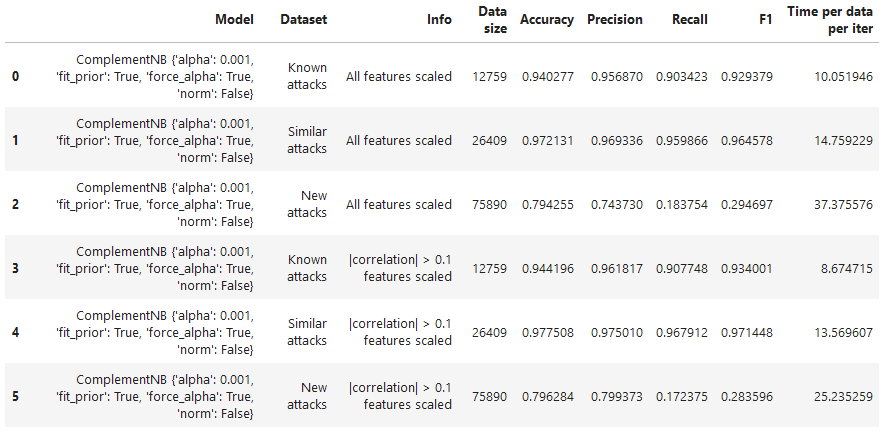
\includegraphics[width=\linewidth]{figures//naive_bayes/comp_nb_bench.png}
    % maybe we can use roc curves instead? they can fit in a single column...?
    \caption{Complement Naive Bayes Benchmark}%ieee caption go on the bottom
    \label{fig:comp_nb_bench}
\end{figure*}
%\lipsum[1]

%\lipsum[1-10]

The results seem as expected, where the model performs well on known and similar attacks, while performing lackluster for new attacks. This test, however, had some issues. The original preprocessing used for the benchmark function used a StandardScaler() and PCA. However, these methods gave negative values, which cannot be used by this model. As a result, the scaling method was changed to MinMaxScaler() and PCA was omitted. But by doing so, the process became different, making comparison a little more difficult, hence why Gaussian Naive Bayes was utilized.

% Could show roc curve here

\subsubsection{Gaussian Naive Bayes}
Gaussian Naive Bayes generally performs better on continuous data, especially that which follows the normal distribution. While the data is not necessarily normal, it is continuous due to the StandardScaler() that is applied for the benchmark function. Unlike ComplementNB(), GaussianNB() is able to use negative values, allowing it to follow the same preprocessing and benchmark tests as the other models. This makes it much easier to make a comparison in terms of overall performance. GaussianNB() has two main parameters: priors, which are the prior probabilties for the classes, and var\_smoothing, which is the portion of the largest variance of all features that is added to variances for stability. In this case, priors was ignored and hyperparameter tuning was only performed based on var\_smoothing. The parameter grid used was \{'var\_smoothing': np.logspace(0,-9, num=100)\}, which creates 100 numbers between 1 and 1e-9.

Featured in Figure \ref{fig:gaus_nb_bench} are the results for Gaussian Naive Bayes,

Featured in Figure \ref{table-gaussiannb-results} are the results for Gaussian Naive Bayes,
% i might have gone overboard with the to_latex function in pandas, but check these
\begin{table}[!htb]
\centering
\resizebox{\linewidth}{!}{\begin{tabular}{llrrrrr}
\toprule
 &  & Accuracy & Precision & Recall & F1 & Time (ms) \\
Pipeline & Dataset &  &  &  &  &  \\
\midrule
\multirow[c]{3}{*}{scaled} & Known & 0.817 & 0.707 & 0.991 & 0.825 & 9.917 \\
 & Similar & 0.795 & 0.661 & 0.987 & 0.792 & 19.195 \\
 & New & 0.691 & 0.313 & 0.268 & 0.289 & 50.295 \\
\cline{1-7}
\multirow[c]{3}{*}{corr, scaled} & Known & 0.826 & 0.716 & 0.995 & 0.833 & 4.697 \\
 & Similar & 0.806 & 0.672 & 0.994 & 0.802 & 7.989 \\
 & New & 0.700 & 0.319 & 0.251 & 0.281 & 28.354 \\
\cline{1-7}
\multirow[c]{3}{*}{PCA} & Known & 0.786 & 0.672 & 0.992 & 0.801 & 15.768 \\
 & Similar & 0.760 & 0.625 & 0.984 & 0.764 & 30.440 \\
 & New & 0.664 & 0.383 & 0.711 & 0.498 & 83.340 \\
\cline{1-7}
\multirow[c]{3}{*}{corr, PCA} & Known & 0.935 & 0.923 & 0.927 & 0.925 & 12.799 \\
 & Similar & 0.969 & 0.943 & 0.980 & 0.961 & 22.165 \\
 & New & 0.793 & 0.729 & 0.186 & 0.296 & 41.312 \\
\cline{1-7}
\bottomrule
\end{tabular}
}
\caption{GaussianNB results}
\label{table-gaussiannb-results}
\end{table}


% This one is the pretty one
\begin{figure}
    \centering
    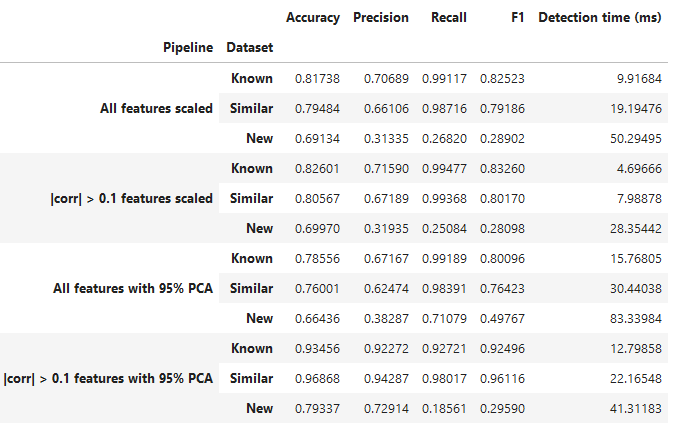
\includegraphics[width=1\linewidth]{figures//naive_bayes/gaus_nb_bench_pretty.png}
    \caption{test}
    \label{fig:enter-label}
\end{figure}
% Benchmark table
% Thats the big one
\begin{figure*}
    \centering
    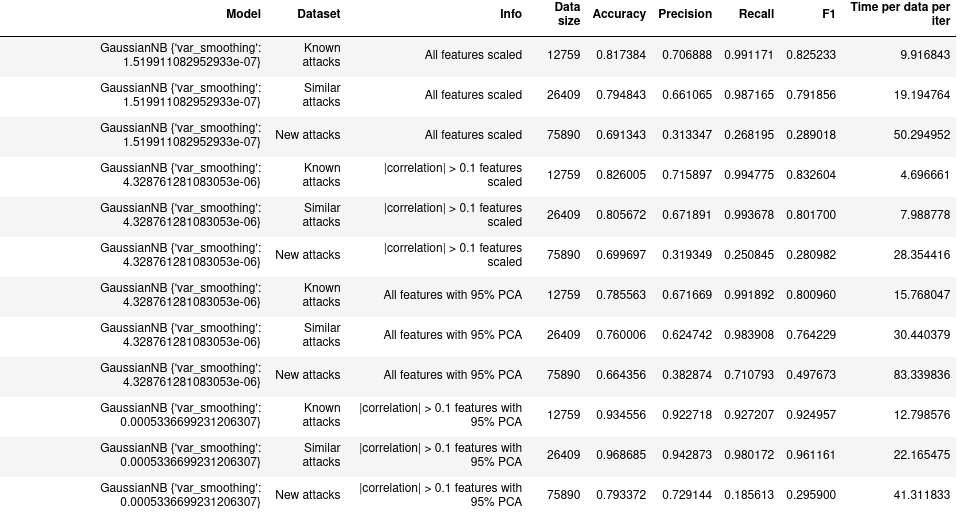
\includegraphics[width=1\linewidth]{figures//naive_bayes/gaus_nb_bench.png}
    \caption{Gaussian Naive Bayes Benchmark}
    \label{fig:gaus_nb_bench}
\end{figure*}

Overall, this model still performed as expected, where the known and similar attacks data performed well while the new attacks performed worse. Based on what can be compared with ComplementNB(), the overall accuracies and computation time are quite comparable with each other. However, the precision to recall ratio is much different. For ComplementNB(), the precision is much greater than the recall whereas for GaussianNB(), they were low but closer to each other. * add more *

The best performing test was using all the features with 95\% PCA.This used a var\_smoothing of 4.328761281083053e-06. In terms of performance with known and similar attacks, it performed around the same, with F1 scores of 0.80096 and 0.76423 respectively. However, the new attacks drastically increased performance in terms of F1 score, achieving an F1 score of 0.49767, which is nearly double of those from the other tests. Despite having a slight accuracy drop, we believe that this is the best performing Naive Bayes model, mainly due to the class imbalance that exists in the data. The precision of the model is approximately the same as the other tests, but the recall is significantly higher, going from around 0.25 to 0.7, implying that it is identifying threats and non threats much better than the others tests.

% Roc curve
Roc curve stuff...
% use 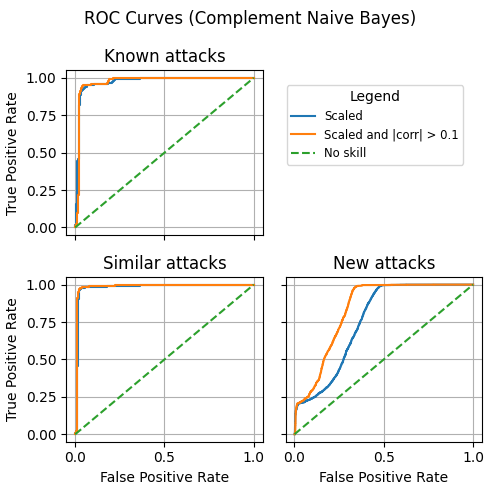
\includegraphics{figures/Complement Naive Bayes_roc_all_small.png}

% My conclusion stuff (the stuff below), or should we just put this in the actual conclusion    

% Do i include this here? I believe that the model performed well (the best among all models) because it is not overfitting as much. The other models seemed to have near 1 accuracy for known and similar, but extremely low for new. Mine on the other hand, has lower acc (80% ish), but achieved 40-50% on new. One thing to note is that naive bayes is considered a generative learning algorthim while the other models are considered discriminative. This means that naive bayes models the distribution of inputs of a given class while discriminatives try to learn which features are most important to differentiate between classes. It's possible that the discriminative models identified certain fetures, causing it them to overfit.

% Also, my best performing model is 95% PCA; the acc severely drops when using correlation 95% PCA. The correlation dropping was based on the known attack dataset. As a result, it is possible that features that were not important for known and similar attacks are very important for new attacks. Due to this, this process likely removed features that were important for new attacks.

\subsection{Support Vector Machines}
\begin{table*}[!htb]
    \centering
    \include{table-partials/svm-results}
    \caption{Caption}
    \label{tab:my_label}
\end{table*}
\subsection{model 3}
\subsection{model 4}
\subsection{XGBoost}
XGBoost is a popular supervised tree based algorithm that is popularly used in classification problems. This model is an example of an ensemble technique which follows the boosting principle. XGBoost is beneficial for several reasons. It tends to deliver a relatively high accuracy. It is also known for being very efficient when making predictions making them suitable for real time applications. XGBoost is not heavily impacted by outliers and is capable of handling both large and imbalanced datasets. The model is resistant to underfitting by default and has built-in parameters that can help to prevent overfitting. Along with the benefits, the model also has some drawbacks. 

\section{Results and comparison}
% Evaluation
% Could just have all of the tables ibrahim made (best f1, precision , recall, time)
% maybe we should just also show what we think is the best overall model

\section{Conclusion}
% talk about results, and issues w/ our process and what not
% Probably also include the deployment thing here

% \begin{figure}[!htb]
%   \centering
%   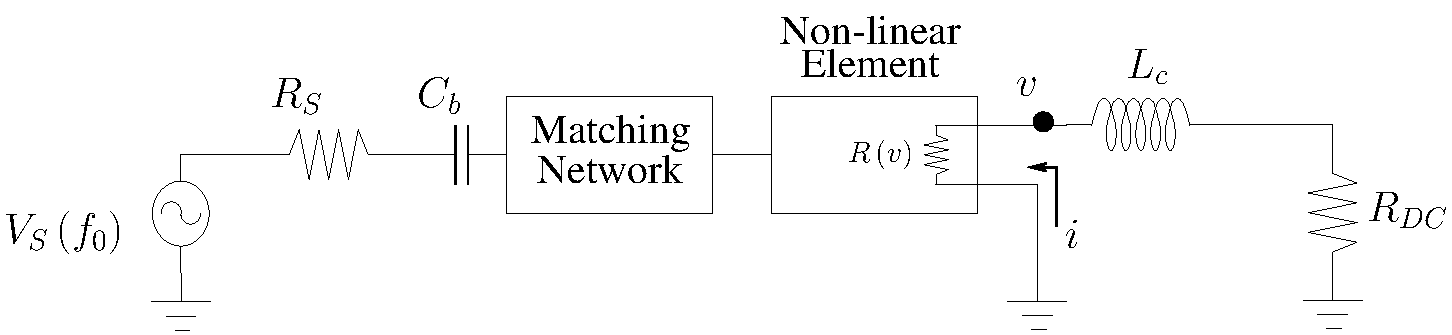
\includegraphics[width=\linewidth]{figures/01.pdf}
%   \caption{This is how to add a figure and caption}
%   \label{circuit_diagram}
% \end{figure}

% This is how to reference a Fig.~\ref{circuit_diagram}.

% This is how to write an equation and reference it like eq. \ref{ideal_rectifier_resistance}.
% \begin{equation}
% \label{ideal_rectifier_resistance}
% R(v) =
% \begin{cases}
%     \infty, & v > 0\\
%     0, & v \leq 0
% \end{cases}
% \end{equation}

% \begin{itemize}
%     \item This
%     \item is
%     \item how to make an unnumbered list
% \end{itemize}


% \begin{enumerate}
%     \item This
%     \item is
%     \item how to make a numbered list
% \end{enumerate}

\ifCLASSOPTIONcaptionsoff
  \newpage
\fi

\bibliographystyle{IEEEtran}
\bibliography{IEEEabrv,Bibliography}

% \begin{IEEEbiography}[{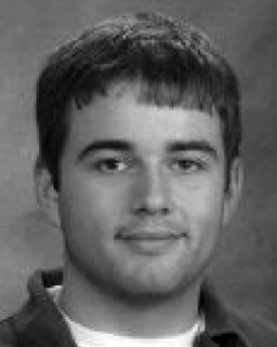
\includegraphics[width=1in,height=1.25in,clip,keepaspectratio]{photo/mike.png}}]{Michael Roberg}
% Do we need a bio section? We should ask the professor
% \end{IEEEbiography}
\vfill
\end{document}